%!TEX root = ./../main.tex
%!TEX encoding = UTF-8 Unicode
%----------------------------------------------------------------------------------------
%   CHAPTER 2
%   translator: InSight
%   proofreader: SI, laserdog
%----------------------------------------------------------------------------------------

\chapterimage{chapter_head_1.pdf} % Chapter heading image



\chapter[狭义相对论]{Special Relativity \quad 狭义相对论}
\label{chap2}
 著名的Michelson-Morley实验告诉我们,光在任何参考系中都具有相同的速度\mpar{日常生活中所观测到的物体的速度取决于选定的参考系。如果一个观察者站在火车站上,测得的火车速度为$50 \mathrm{km\,h^{-1}} $,另一个观察者以$15\mathrm{km\,h^{-1}}$ 的速度与火车一同运动,那么测得的火车速度就应是$35 \mathrm{km\,h^{-1}}$。与此不同的是,光始终以$1.08 \times 10^9 \mathrm{km\,h^{-1}}$运动,不论如何相对于光运动。}。Albert Einstein首先意识到这个结果所蕴含的深刻意义,从而在此基础之上建立了狭义相对论。从光速不变原理出发,Einstein预言了许多有趣而又悖于常理的现象,最后都被实验证实是正确的。在这里我们首先阐明狭义相对论的基础,然后再体会这个原理的强大之处。狭义相对论有两个基本假设:
 \begin{itemize}
   \item {\bf{相对性原理:}} 任意惯性系,即任意两个相对速度恒定的参考系的物理规律相同。
   \item {\bf{光速不变原理:}} 在任意惯性系中的光速均为常数$c$。
 \end{itemize}
除此之外,我们还假设时空均匀且各向同性。这意味着不论在哪儿(均匀),不论朝着什么方向(各向同性)做实验,物理规律都是一样的。例如两个物理学家,一个在纽约,一个在东京,他们做完全一样的两个实验,会得到相同
\mpar{这当然要排除某些参数的影响,例如重力加速度。}  的物理规律,就算是在火星也一样。

%翻译欠佳,主语应该换换
正确的物理定律不应该随看实验的角度%这里我不太确定
或是进行实验的时间点而变。\footnote{原文为:The laws of physics, formulated correctly, shouldn't change if you look at the experiment from a different perspective or repeat it tomorrow.}此外,狭义相对论的第一条假设告诉我们,不管是在匀速运动的马车上,还是是在静止的实验室中,做同一物理实验都会得到相同的结果。以上论述均与与我们的生活经验相符。举个例子,如果你闭着眼睛坐在匀速运动的汽车上,你是没有办法分辨出你是真的在运动还是静止的。

如果没有了各向同性和均匀性,物理学就会遇到很大的麻烦:从实验中得到的物理定律如果仅仅在空间中的某一点对于确定的某一方向成立,显然是毫无用处的。

唯一有些不直观的就是狭义相对论的第二条假设,毕竟它违背了我们所有的日常经验。虽然如此,至今为此所有的实验都表明这个假设是正确的。
\section[狭义相对论的中的不变量]{The Invariant of Special Relativity \quad 狭义相对论的中的不变量}
\label{sec2.1}
在接下来的几节中,我们将使用狭义相对论的两个基本假设推导出Minkowski度规,有了它,我们就能计算两个物理事件的“距离”。物理事件在这里指在Minkowski 时空中的点,而整个狭义相对论都建立在Minkowski时空之上。我们从而得知任意两个不同惯性参考系之间的变换必须保证Minkowski度规不变,通过这一条件我们能够找到连接两个允许存在的惯性系(也就是光速为常数的参考系)之间所有的变换\footnote{非常类似我们要找旋转变换对应的各个参数的变换规律,而旋转变换保证了长度的守恒}。
在本书其余的部分我们将会用到这些关于变换的知识,来寻找在这些变换下不变的方程。让我们从一个能导出一条狭义相对论假设的最重要的推论之一的思想实验开始。
{\marginpar{
    \centering
    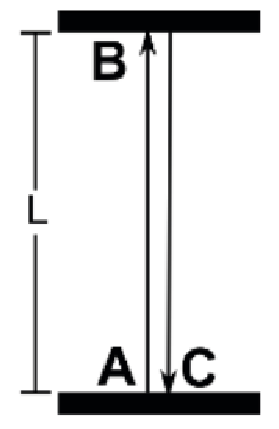
\includegraphics[scale=0.5]{fig2_1.pdf}
    \figcaption{思想实验图示}
    \label{fig2.1}
}}
设想坐标系中一观察者,在原点处向上发出一个光脉冲,经过一段时间后被垂直镜面反射回原点。如图\ref{fig2.1}所示

有3个重要的事件:
\begin{itemize}
  \item {\bf{A:}}光从原点发出
  \item {\bf{B:}}光在镜面上反射
  \item {\bf{C:}}光回到原点
\end{itemize}
事件{\bf{AC}}之间的时间间隔为\mpar{对于恒定速度$v$而言,有$v=\frac{\Delta s}{\Delta t}$,$\Delta s$表示经过的距离,$\Delta t$代表所需时间,因此$\Delta t=\frac{\Delta s}{v}$}
\begin{equation}\label{equ2.1}
\Delta t=t_C-t_A=\frac{2L}{c}
\end{equation}
式中$L$表示原点与反射点之间的距离。

{\marginpar{
        \centering
        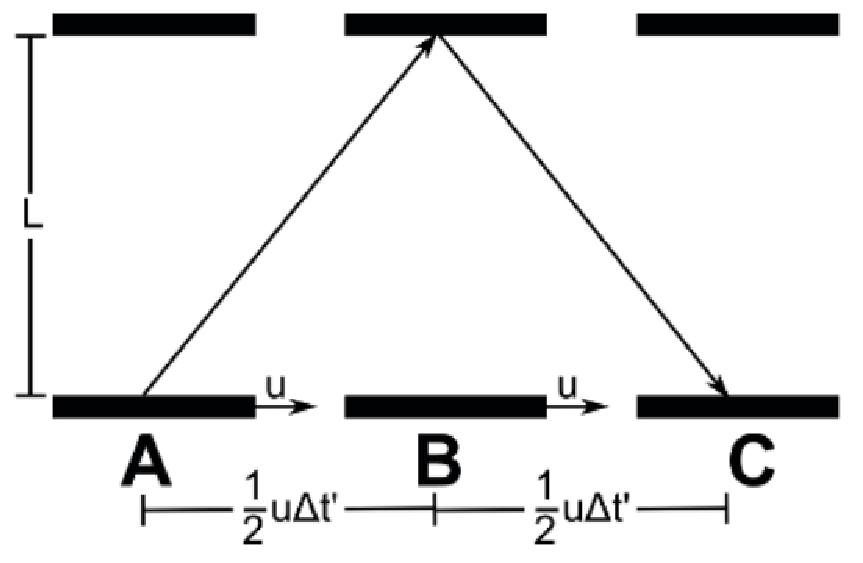
\includegraphics[scale=0.31]{fig2_2.pdf}
        \figcaption{思想实验图示. 第二位移动观察者向左移动, 因此第一位观察者相对他向右移动}
        \label{fig2.2}
}}


接下来考虑第二位观察者,在$t_A$时刻处于他所在的坐标系的原点,并以恒定速度$u$相对于第一个观察者\mpar{那些能将两相对速度恒定的惯性参考系中的物理量相互转化的变换称为
{\bf{推动(Boost)}}变换, 后面我们会对此进行详述。}向左运动。为简便起见,我们假设第二个参考系的原点在$t_A$时刻与第一位观察者的坐标系原点重合。第二位观察者所见到的现象就与第一位不一样了。在他的参考系中,光脉冲的起点和终点并不在同一位置(见图\ref{fig2.2})。

用数学语言表示:
\begin{equation}\label{equ2.2}
  x'_A=0 \neq x'_C=u \Delta t' \qquad \rightarrow \qquad \Delta x' =u \Delta t'
\end{equation}
带撇物理量代表第二位观察者所测量的量。对于第一位静止系的观察者而言有
\begin{equation}\label{equ2.3}
  x_A=x_C \qquad \rightarrow \qquad \Delta x=0
\end{equation}
假定了第二位观察者运动沿$x$轴,因此
\begin{equation}\label{equ2.4}
 y'_A=y'_C \quad  \quad z'_A=z'_C \quad \rightarrow \quad \Delta y'=0 \quad  \quad \Delta z'=0
\end{equation}
那么同样也有
\begin{equation}\label{equ2.5}
 y_A=y_C \quad  \quad z_A=z_C \quad \rightarrow \quad \Delta y=0 \quad  \quad \Delta z=0
\end{equation}

接下来的问题是:{\bf{第二位观察者所测得的时间间隔是多少?}}因为已经假定了光速为常数,那么事件{\bf{AC}}对于第二位观察者而言将具有不同的间隔!时间间隔$\Delta t'=t'_C-t'_A$,等于光在第二位观察者的参考系中走过的距离$l$除以光速$c$。
\begin{equation}\label{equ2.6}
  \Delta t'=\frac{l}{c}
\end{equation}
我们可以利用古老的Pythagoras\footnote{通译为毕达哥拉斯。}定理(见图\ref{fig2.2}) 计算光传播的距离
\begin{equation}\label{equ2.7}
  l=2 \sqrt{\left(\frac{1}{2} u \Delta t'\right)^2+L^2}
\end{equation}
利用式\eqref{equ2.6}可以得到
\begin{equation}\label{equ2.8}
  c \Delta t' =2 \sqrt{\left(\frac{1}{2} u \Delta t'\right)^2+L^2}
\end{equation}
再利用式\eqref{equ2.2}中的$\Delta x'=u\Delta t'$可得
\begin{displaymath}
c \Delta t' =
  2 \sqrt{\left(\frac{1}{2} u \Delta t'\right)^2+L^2}
\end{displaymath}
\begin{displaymath}
  \rightarrow
  \left( c \Delta t' \right)^2 =
   4 \left( \left(\frac{1}{2} u \Delta t'\right)^2+L^2 \right)
\end{displaymath}
\begin{equation}\label{equ2.9}
\rightarrow
\left( c \Delta t' \right)^2
-\left(\Delta x' \right)^2=
4 \left( \left(\frac{1}{2} u \Delta t'\right)^2+L^2 \right)
-\left(\Delta x' \right)^2 =4L^2
\end{equation}
 现在回到式\eqref{equ2.1},即$\Delta t =\frac{2L}{c}$,那么
\begin{equation}\label{equ2.10}
 \left( c \Delta t' \right)^2
 -\left(\Delta x' \right)^2
 =4 L^2
 =\left( c \Delta t \right)^2
 =\left( c \Delta t \right)^2
 -
 \!\!\!
 \underbrace{\left(\Delta x \right)^2}_{=0 \text{由式}\eqref{equ2.3} \text{知}}
\end{equation}
终于,我们得到\mpar{\it{注意到我们在此处采用的是得到这个结果的最简方法,因为我们假定$t_A$时刻两坐标的原点是重合的。尽管如此,就算我们任意选择两惯性参考系原点的关系,仍然可以证明这个结论,只是过程会复杂一些。因为物理定律在任意惯性系中都是一样的,这给了我们任意选择便于计算的参考系的自由。如果第二位观察者的参考系运动方向是任意的,那就不再有$\Delta y'=0$和$\Delta z'=0$,但虽然如此,我们能够证明方程仍然是成立的,因为物理定律在任意惯性系中都是一样的。$^{\color{red}{4}}$\ \\ \ \\ {$^{\color{red}{4}}$ 译者注:原文的确把这句话说了两遍}}}

\begin{equation}\label{equ2.11}
\left( c \Delta t' \right)^2
-\left(\Delta x' \right)^2
-\underbrace{\left(\Delta y' \right)^2}_{=0}
-\underbrace{\left(\Delta z' \right)^2}_{=0}
=
\left( c \Delta t \right)^2
-\underbrace{\left(\Delta x \right)^2}_{=0}
-\underbrace{\left(\Delta y \right)^2}_{=0}
-\underbrace{\left(\Delta z \right)^2}_{=0}
\end{equation}
考虑第三个观察者,相对于第一个观察者以不同的速度运动,用同样的推理可以得到
\begin{equation}\label{equ2.12}
\left( c \Delta t'' \right)^2
-\left(\Delta x'' \right)^2
-\left(\Delta y'' \right)^2
-\left(\Delta z'' \right)^2
=
\left( c \Delta t \right)^2
-\left(\Delta x \right)^2
-\left(\Delta y \right)^2
-\left(\Delta z \right)^2
\end{equation}
因此,我们得到了一些对于所有观察者都相同的量:即二次型
\begin{equation}\label{equ2.13}
(\Delta s)^2
\equiv\left( c \Delta t \right)^2
-\left(\Delta x \right)^2
-\left(\Delta y \right)^2
-\left(\Delta z \right)^2
\end{equation}

此外,我们还能看出对于不同观察者,$(\Delta x)^2+(\Delta y)^2+(\Delta z)^2$或者说$(c\Delta t)^2$是不同的。我们将在下一节讨论不变量$\Delta s^2$所蕴含的物理意义。


\section[固有时]{Proper Time \quad 固有时}
\label{sec2.2}
我们在上一节推导出了狭义相对论中的不变量$\Delta s^2$,其在所有观察者眼中都相同。接下来我们要讨论这个量的物理意义。
    \marginpar{
        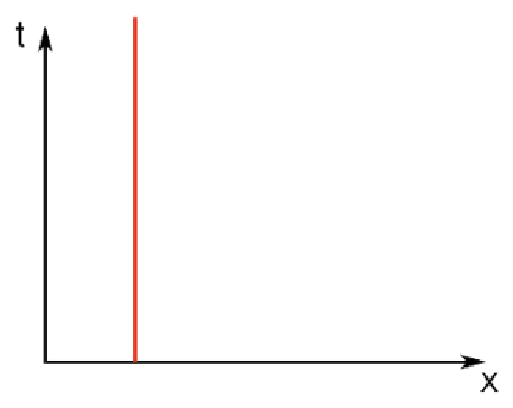
\includegraphics[scale=0.4]{fig2_3.pdf}
        \figcaption{静止物体的世界线。物体位置不随时间流逝而变化。}\label{fig2.3}
    }
为简便起见,我们将问题限制在一维空间中。对于一个相对于观察者静止的物体,我们能作出它的时空图(见图\ref{fig2.3})。相应的,一个匀速运动的物体能作出如图\ref{fig2.4}所示的时空图。

    \marginpar{
        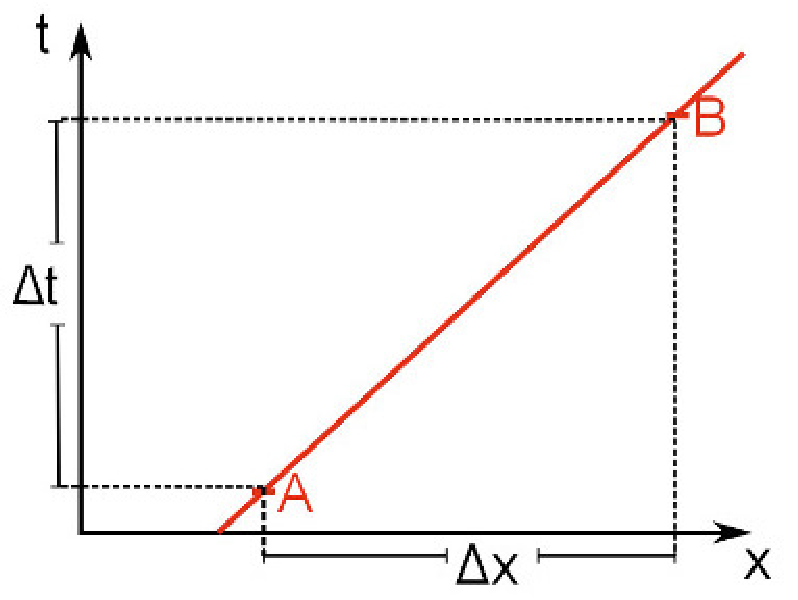
\includegraphics[scale=0.35]{fig2_4.pdf}\label{fig2.4}
        \figcaption{某匀速直线运动物体的世界线。物体前后经过某两点记为事件A,B。它们间的空间距离为$\Delta x$,时间间隔为$\Delta t$}
    }
我们画来用于确定物体在时空中位置的线称为{\bf{世界线(world line)}}。世界线总是依赖于观察者的。两不同观察者对于同一物体可能会画出完全不同的世界线。若一观察者眼中的物体时空图为图\ref{fig2.4},那么对于速度与物体相同的观察者,其时空图将为图\ref{fig2.5},即对于此观察者物体静止。为了解释两位观察者给出的不同描述,我们引入$x'$ 和$t'$ 表示第二位观察者的参考系中的时间和位置。\footnote{注意:我们这里使用的例子与节\ref{sec2.1}不同}

我们可以看到,两个观察者将对事件$AB$之间的变化持不同观点。对于第一位观察者,$\Delta x \neq 0$, 但对于第二位观察者,$\Delta x' = 0$。 两观察者都认为事件$A$ 和$B$ 之间的时间间隔非零:$\Delta t \neq 0$ 和$\Delta t' \neq 0$,且认为$\Delta s^2$也相同(见上节推导的结论,任意观察者都有相同的$\Delta s^2$)。 这将导出一个令人惊讶的结论:事件$A$ 到$B$ 经历的时间对于两观察者不同
    \marginpar{
        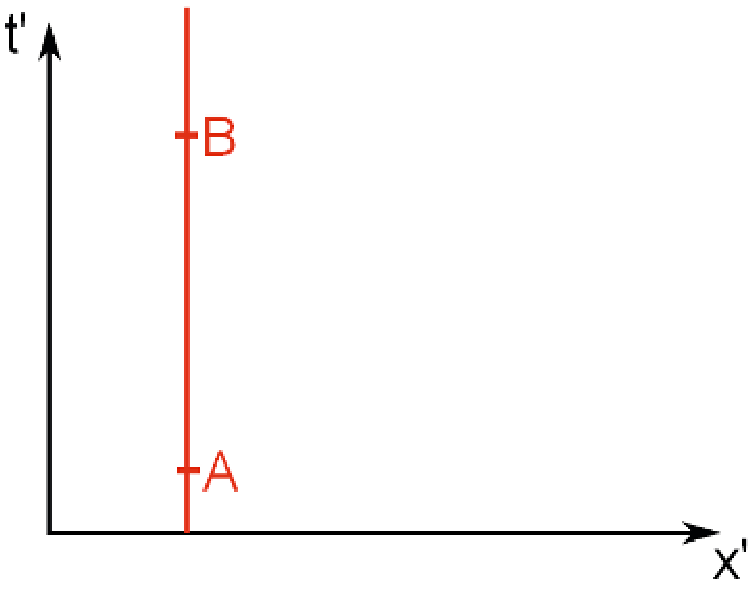
\includegraphics[scale=0.35]{fig2_5.pdf}
        \figcaption{同一个运动物体的世界线,但观察者与该物体速度相同。该观察者观测到的事件AB之间的空间距离为$\Delta x' = 0$}\label{fig2.5}
    }
\begin{equation}\label{equ2.14}
  (\Delta s)^2
  =(c\Delta t)^2
  -(\Delta x)^2
\end{equation}
\begin{equation}\label{equ2.15}
  (\Delta s')^2
  =(c\Delta t')^2
  -\underbrace{(\Delta x')^2}_{=0}
  =(c\Delta t')^2
\end{equation}
\begin{equation}\label{equ2.16}
   (\Delta s)^2
   = (\Delta s')^2
   \rightarrow
    (\Delta t')^2 \neq
     (\Delta t')^2
     \quad \text{因为}  (\Delta x)^2 \neq 0
\end{equation}

这是有关狭义相对论最著名的一个效应,通常称为{\bf{钟慢效应(time-dilation)}}。时间间隔依赖于观察者,正如空间距离一样。不同观察者时间流逝速度不同,因此两事件经历的时间也就自然不同了。

现在时间将变为一个相对的概念,如果我们能找到一个对于所有观察者都相同的时间量,这将会非常有用。在上述例子中,第二位观察者与物体有相同的速度,有
\begin{equation}\label{equ2.17}
  (\Delta s')^2
  =(c\Delta t')^2
\end{equation}

上式意味着狭义相对论中的不变量恰为观察者所观测到的时间间隔乘上光速$c$。这让我们有机会能用$(\Delta s)^2$定义一个对于所有观察者相同的时间量。我们定义
\begin{equation}\label{equ2.18}
  (\Delta s)^2
  =(c\Delta \tau)^2
\end{equation}
$\tau$称为{\bf{固有时(proper time)}}。固有时是所有相对于该物体静止的观察者所测量的时间。

当然,现实生活中的物体绝非只能做匀速运动,但我们可以取足够短的时间(无穷小),使得运动近似为匀速运动,这样固有时的概念就说得通了。因此数学上我们需将概念过渡到无穷小,即$\Delta \rightarrow d$:
\begin{equation}\label{equ2.19}
  (ds)^2  =(cd \tau )^2=(cdt)^2-(dx)^2-(dy)^2-(dz)^2
\end{equation}

因此,就算一个物体到处乱跑,我们也能假设一个与物体一起运动的自带时钟的观察者,这样他总与该物体相对静止。对于这个特定的观察者而言,他所测量的时间间隔就是固有时,这一数值对其余观察者也是相同的,因为$(ds)^2=(cd\tau)^2$对于任意观察者成立。再次强调,这并不意味着对所有观察者都有同样的时间间隔,只是这些观察者承认该特殊观察者所测量的时间间隔为一不变量罢了。

\section[速度上限]{Upper Speed Limit \quad 速度上限}
\label{sec2.3}
在上节中我们对狭义相对论这一不变量有了解释,现在可以更进一步,导出另一个狭义相对论的惊人结论。

由于不变量的定义中带有负号,这意味着对于时空中的两个事件,$(\Delta s)^2$的值可能为0。$(\Delta s)^2$的值甚至可能是负的,但这样我们将得到一个复的固有时\mpar{按固有时定义,$(ds)^2=(cd\tau)^2$,$(ds)^2 < 0 \rightarrow d\tau$ 为复数。},通常复的固有时没有物理意义。因此,$(\Delta s)^2=0$时固有时最小,$\tau=0$,令
\[
\Delta s^2_{min}
=0=(c \Delta t)^2-(\Delta x)^2-(\Delta y)^2-(\Delta z)^2
\]
\[
\rightarrow (c \Delta t)^2
=(\Delta x)^2+(\Delta y)^2+(\Delta z)^2
\]
\begin{equation}\label{equ2.20}
 \rightarrow c^2=
  \frac{(\Delta x)^2+(\Delta y)^2+(\Delta z)^2}{(\Delta t)^2}
\end{equation}
在上式右侧我们有速度平方$v^2$,也就是距离除上时间,把这个式子写成极限,则
\begin{equation}\label{equ2.21}
 \rightarrow c^2=\frac{(d x)^2+(d y)^2+(d z)^2}{(dt)^2}
\end{equation}
函数$x(t)$,$y(t)$,$z(t)$是描述两事件之间路径的参数方程,这样式子右侧就是两事件间的运动速率。
%flag 此处的速度在文中并无主语,可能要加上物体二字,那么前面也得改。

因此,当某一观察者测得的固有时为$0$时其速度将满足下式
\begin{equation}\label{equ2.22}
  \rightarrow c^2 =v^2
\end{equation}
这意味着没有物体能以超过光速$c$的速度运动!\footnote{译者注:否则其固有时为复}{\bf{我们给物理学中的一切事物找到了一个速度上限。}}时空中的两事件相互影响的传播速度不能超光速。

{\it{这一点满足物理学上的{\bf{局域性原理(principle of locality)}},即物理学中的对象只能被它邻近的对象影响。相互作用都是局域的,不存在超距作用,物理效应的传播需要时间。}}

\section[Minkowski记法]{The Minkowski Notation \quad Minkowski 记法}
\label{sec2.4}
\begin{quote}
从现在起,孤立的空间和孤立的时间注定要消失成为影子,只有两者的统一才能保持独立的存在。
\end{quote}
\begin{flushright}
  {\bf{-Hermann Minkowski}}\mpar{出自Hermann Minkowski在Assembly of German Natural Scientists and Physicians(1908.9.21)上的演讲}
\end{flushright}
写出狭义相对论中不变量
\begin{equation}\label{equ2.23}
 ds^2=(cdt)^2-(dx)^2-(dy)^2-(dz)^2
\end{equation}
在此处将采用一种新的记法,这种记法初学时可能稍显复杂,不过后文中将经常用到:\\
\begin{align}
ds^2&=\eta^{\mu\nu}dx_\mu dx_\nu \notag \\
&=\eta^{00}(dx_0)^2+\eta^{11}(dx_1)^2+\eta^{22}(dx_2)^2+\eta^{33}(dx_3)^2 \notag \\
&=dx_0^2-dx_1^2-dx_2^2-dx_3^2\notag \\
&=(cdt)^2-(dx)^2-(dy)^2-(dz)^2 \label{equ2.24}
\end{align}
在这里我们用了一些新的约定和记号,这些东西在近代物理中应用很广泛,所以越早熟悉越好:
\begin{itemize}
  \item Einstein求和约定:某指标在同一项内出现两次则代表遍历该指标并求和。例如:$\sum_{i=1}^3a_i b_i =a_i b_i=a_1 b_1 +a_2 b_2 +a_3 b_3$,但$\sum_{i=1}^3a_i b_j=a_1 b_j +a_2 b_j +a_3 b_j\neq a_i b_j$
  \item 像$\mu$,$\nu$,$\sigma$这样的希腊字母
  \mpar{像 $i$,$j$,$k$这样的罗马字母作指标时一般代表从1到3求和:$x_i x_i \equiv \sum_i^3 x_i x_i$。 后面我们还会用到大写的罗马字母如$A$,$B$,$C$,它们作指标时代表从1到8求和。} 作指标时,一般代表从0 到3 求和:$x_\mu y_\mu=\sum_{\mu=0}^3 x_\mu y_\mu $
  \item 我们约定变量$x_0\equiv ct$,$x_1\equiv x$,$x_2\equiv y$,$x_3\equiv z$。这样时间空间地位等同,也便于我们使用Einstein求和约定
  \item 引入Minkowski度规($\eta$看作一矩阵,$\eta^{ij}$ 为其矩阵元):$\eta^{00}=1$,$\eta^{11}=-1$,$\eta^{22}=-1$,$\eta^{33}=-1$,当$\mu \neq \nu$时$\eta^{\mu\nu}=0$  (也可以等价的写为
\mpar{$\eta^{\mu\nu}= \\ \\
       \left(
       \begin{array}{cccc}
        1 & 0 & 0 & 0 \\
         0 & -1 & 0 & 0 \\
          0 & 0 & -1 & 0 \\
          0 & 0 & 0  & -1\\
        \end{array}
        \right)$ }
      $\eta^{\mu\nu} = \mathrm{diag} (1,-1,-1,-1)$)
\end{itemize}

另外按常规我们还要引入{\bf{四维矢量(four-vector)}},简称{\bf{4矢}}。
\begin{equation}\label{equ2.25}
  dx_\mu =\left(\begin{array}{c}
            dx_0 \\
            dx_1 \\
            dx_2 \\
            dx_3
          \end{array}\right)
\end{equation}
式\eqref{equ2.24}可用4矢和Minkowski度规表出
\begin{align}
  &(ds)^2=dx_\mu \eta^{\mu\nu} dx_\nu \notag \\
  &=\left(
     \begin{array}{cccc}
       dx_0 & dx_1 & dx_2 & dx_3 \\
     \end{array}
   \right)
   \!\!\!
   \left(
     \begin{array}{cccc}
       1 & 0 & 0 & 0 \\
       0 & -1 & 0 & 0 \\
        0 & 0 & -1 & 0 \\
        0 & 0 & 0  & -1\\
     \end{array}
   \right)
   \!\!\!
   \left(
     \begin{array}{c}
       dx_0 \\
        dx_1 \\
       dx_2 \\
        dx_3\\
     \end{array}
   \right)\notag \\
   &=dx_0^2-dx_1^2-dx_2^2-dx_3^2 \label{equ2.26}
\end{align}

采用这种记法能让我们省不少事。对于$ds$,我们给出的解释是时空(Minkowski时空)中两事件的“距离”,这个“距离”并不只是空间距离,它还将时间间隔考虑在内。如果我们考虑3维Euclidean 空间\mpar{3维Euclidean空间就是经典物理中一般的空间,在此空间中我们将时间和空间分别处理,也就是未将时空考虑成一个整体的几何结构来考虑。但一旦将时间作为新坐标,结合出时空的观念,我们便能将时间空间放在同一坐标下考虑。}中两点间最短距离的平方\mpar{Kronecker函数$\delta_{ij}$即是单位矩阵在指标记法下的表示,详见附录\ref{appendix.B.5.5}}
\begin{align}
  (ds)^2&=dx_i \delta^{ij} dx_j \notag \\
            &=\left(
               \begin{array}{ccc}
                dx_1 & dx_2 & dx_3 \\
               \end{array}
               \right)
               \left(
               \begin{array}{ccc}
                1 & 0 & 0  \\
                0 & 1 & 0  \\
                0 & 0 & 1  \\
              \end{array}
              \right)
              \left(
              \begin{array}{c}
               dx_1 \\
               dx_2 \\
               dx_3\\
              \end{array}
              \right)\notag \\
           &=(ds)^2=(dx_1)^2+(dx_2)^2+(dx_3)^2\label{equ2.27}
\end{align}

这种数学工具叫{\bf{度规(metric)}},它能够告诉我们无限临近的两点之间的距离。在Euclidean空间中度规就是单位矩阵$\delta_{ij}$。在广义相对论的弯曲时空中将会有更复杂的度规,但在狭义相对论中我们采用的是相对简单的Minkowski度规$\eta^{\mu\nu}$。度规是计算长度的工具,我们可以通过度规定义{\bf{4矢的长度(length of a four-vector)}},即4矢与自身的标量积\mpar{此定义在Euclidean空间中同样适用:由于度规为
$\delta_{ij}=\left(
 \begin{array}{ccc}
 1 & 0 & 0  \\
  0 & 1 & 0  \\
  0 & 0 & 1  \\
  \end{array}
  \right)
$,易得矢量$\vec{v}$的长度$=\vec{v}\cdot\vec{v}=v_1^2+v_2^2+v_3^2$。}
\[
x^2=x \cdot x \equiv x_\mu x_\nu \eta^{\mu\nu}
\]
类似地,两任意4矢的标量积定义为
\begin{equation}\label{equ2.28}
  x\cdot y\equiv x_\mu y_\nu \eta^{\mu\nu}
\end{equation}

对于上下标,也有一些约定能使计算过程更清晰。我们定义带有 上指标的4矢\mpar{带有下指标的4矢通常叫做协变4矢,带有上指标的4 矢通常叫做逆变4矢。}
\begin{equation}\label{equ2.29}
  x^{\mu}\equiv\eta^{\mu\nu}x_\nu
\end{equation}
或者
\begin{equation}\label{equ2.30}
  y^{\nu}\equiv\eta^{\mu\nu}y_\mu
 \!\!\!\!\!\!\!\!\!\!\!\!\!\!\!\!\!\!\!\!\!\!\!\!\!\!\!\!
 \underbrace{=}_{Minkowski\text{度规是对称的}\eta^{\mu\nu}=\eta^{\nu\mu}}
 \!\!\!\!\!\!\!\!\!\!\!\!\!\!\!\!\!\!\!\!\!\!\!\!\!\!\!\!
  \eta^{\nu\mu}y_\mu
\end{equation}
因此,标量积可以写为\mpar{指标的名称如何选取并不影响最后的值,详见附录\ref{appendix.B.5.1}。}
\begin{equation}\label{equ2.31}
  x\cdot y\equiv x_\mu y_\nu \eta^{\mu\nu}=x_\mu y^\mu=x^\nu y_\nu
\end{equation}
上式中,变换的上指标是可以任意选择的,这只是为了避免公式中总是出现$\eta^{\mu\nu}$的一种方法,正如引入Einstein求和约定是为了避免总是出现求和号一样。

\section[Lorentz变换]{Lorentz Transformations \quad Lorentz变换}
\label{sec2.5}
下一步,我们将尝试找出两参考系之间不违背狭义相对论基本假设的变换方式。由上文可知,从狭义相对论的两个基本假设可以推出对于所有惯性参考系均有$ds^2=\eta^{\mu\nu} dx_\mu dx_\nu $,即
\begin{equation}\label{equ2.32}
  ds'^2= dx'_\mu dx'_\nu \eta^{\mu\nu}
  =ds^2
  =dx_\mu dx_\nu\eta^{\mu\nu}
\end{equation}
因此,两参考系间所允许的变换要能保证这个二次式的形式,和Minkowski时空中的标量积在变换下不变。设变换为$\Lambda$,那么变换后
\begin{equation}\label{equ2.33}
  dx_\mu \rightarrow dx'_\mu=\Lambda^\sigma_\mu dx_\sigma
\end{equation}
由于$(ds)^2$在变换下不变
\begin{align}
(ds)^2&=(ds')^2 \notag\\
\rightarrow dx\cdot dx &\overset{\text{!}}{=} dx' \cdot dx' \notag \\
\rightarrow dx_\mu dx_\nu\eta^{\mu\nu} &\overset{\text{!}}{=} dx'_\mu dx'_\nu\eta^{\mu\nu} \underbrace{=}_{\mathclap{\eqref{equ2.33}\text{式}}} \Lambda_\mu^\sigma dx_\sigma \Lambda_\nu^\gamma dx_\gamma\eta^{\mu\nu}\notag \\
\underbrace{\rightarrow}_{\mathclap{\text{重命名哑指标}}} dx_\mu dx_\nu\eta^{\mu\nu} &\overset{\text{!}}{=} \Lambda^\mu_\sigma dx_\mu \Lambda^\nu_\gamma dx_\nu\eta^{\sigma\gamma}\notag\\
\underbrace{\rightarrow}_{\mathclap{因为dx_\nu\text{任意}}} \eta^{\mu\nu} &\overset{\text{!}}{=} \Lambda^\mu_\sigma\Lambda^\nu_\gamma\eta^{\sigma\gamma}\label{equ2.34}
\end{align}
或者用矩阵形式来写\mpar{详见附录\ref{appendix.C.1}。}
\begin{equation}\label{equ2.35}
  \eta=\Lambda^{\mathrm{T}}\eta\Lambda
\end{equation}

{\bf{此即变换$\Lambda_\mu^\nu$所需满足条件。}}

这个条件现在看起来可能有些奇怪,但在后文中我们会用更自然的方式导出这个条件。在下一章里,我们会看到Euclidean空间中的旋转所导出的变换%
\mpar{稍后会讲明$O$的意义。}$O$能够保证Euclidean 空间的标量积不变\mpar{“$\cdot$”表示的是矢量的点乘,如果我们将矢量写为列向量,那么按矩阵相乘的定义有$\vec{a}\cdot\vec{b}=\vec{a}^\mathrm{T}\cdot\vec{b}$。 有关$(Oa)^\mathrm{T}=a^\mathrm{T}O^\mathrm{T}$这一点详见附录\ref{appendix.C.1},式\ref{equC.3}。}% 此处原文有误
\begin{equation}\label{equ2.36}
  \vec{a} \cdot \vec{b}
  \overset{\text{!}}{=}
  \vec{a'} \cdot \vec{b'}
  \!\!\!\!\!\!\!\!\!\!
  \underbrace{=}_{\text{注意}
  (Oa)^\mathrm{T}=a^\mathrm{T}O^\mathrm{T}}
  \!\!\!\!\!\!\!\!\!\!
  \vec{a}^\mathrm{T} O^\mathrm{T} O\vec{b}
\end{equation}
因此
\mpar{这一条件一般称为{\bf{正交性(orthogonality)}}条件,因此用字母$O$表示。满足$O^\mathrm{T} O={\bf{1}}$的矩阵称为正交矩阵,因为它列与列之间是正交的。换句话说,矩阵的每一列都可以看做一个矢量,正交性条件就是说这些矢量相互正交。}

$O^\mathrm{T} {\bf{1}} O\overset{\text{!}}{=}{\bf{1}}$,恰巧Euclidean 空间的度规就是单位矩阵${\bf{1}}$,其地位正如Minkowski 度规在式\eqref{equ2.35} 中一样。这个性质是旋转的定义中的一部分,旋转不能改变矢量的长度,即在数学上保证标量积不变
\mpar{矢量的长度即是矢量与自身的标量积的平方根。}$^{,}$\footnote{译者注:$\vec{a}\cdot \vec{b}=\frac{1}{2} [(\vec{a}+\vec{b})^2-\vec{a}^2-\vec{b}^2]$,若保证模长不变,标量积也不变。}此外我们还注意到旋转不改变坐标系的手向\mpar{详见附录\ref{appendix.A.5}。},这表明 $\text{det}(O) \overset{\text{!}}{=}1$,因为保证标量积不变的变换除了旋转变换还有空间反演\mpar{空间反演可简单地理解为映射$\vec{x}\rightarrow -\vec{x}$。这种变换满足$\text{det}(O) \overset{\text{!}}{=}$及$O^{\mathrm{T}}O={\bf{1}}$。 因此,如果我们要将变换限制为旋转变换,就需要加上条件$\text{det} (O) \overset{\text{!}}{=} {\bf{1}}$。此外,空间反演变换又称宇称变换。}。

我们定义保Minkowski时空中标量积不变的变换为
{\bf{Lorentz变换(Lorentz transformations)}}
,这也是为保证狭义相对论的假设所必需的。相应的,每当我们需要得到在Lorentz变换下不变的项时,{\it{都必须结合上下指标}}:$x_\mu y^\mu=x_\mu y_\nu \eta^{\mu\nu}$。
在学会一些非常优雅的技术来处理这样的情况之后,我们会在下一章构建这些转换具体的矩阵形式。


\section[不变性,对称性,协变性]{Invariance, Symmetry and Covariance 不变性,对称性,协变性}
在继续之前,我们有一些重要的概念要事先声明。首先,一个量能被称为{\bf{不变量(invariant)}},这个量必须在变换下不变。比如说,我们考虑一个依赖于不同参数$A,B,C,\dots$的任意函数$ F$,$F=F(A,B,C,\dots)$,如果我们将$A,B,C,\dots$变换为$A',B',C',\dots$,有
\begin{equation}\label{equ2.37}
  F(A',B',C',\dots)=F(A,B,C,\dots)
\end{equation}
那么$F$称为变换下的一个不变量。我们可以用对称性来描述。
{\bf{对称性(symmetry)}}是指在某一变换下或者某一系列变换下保持不变的性质。举个例子,如果说一个物理系统在任意的旋转变换下不变,那么该系统具有旋转对称性。再比如说,一间室温为常温的房间,房间内各点的温度与位置无关,换言之,如果把所有的点朝着某特定方向平移一段距离,室温不变。因此我们说室温具有{\it{平移对称性}}。

协变性与不变性有共通之处而又不同。如果一个方程在变换下形式不变,那么称这个方程具有协变性。例如下面这个式子
\[
E_1=a A^2+bBA'+cC^4
\]
在变换之后这个方程写为
\[
E'_1=a A'^2+bB'A'+cC'^4
\]
那么这个方程具有协变性,因其在变换下形式不变。另一方程
\[
E_2=x^2+4axy+z
\]
若在变换之后写为
\[
E'_2=y'^3+4az'y'+y'^2+8z'x'
\]
那么它就不是协变的,因为其形式已经变化。

所有的物理规律都应具有Lorentz协变性\footnote{即在Lorentz变换下具有协变性——译者(InSight)},因为只有这样的物理规律才能在任意参考系下成立。非协变的物理规律只能在某一特定参考系下成立,这会导致在东京和纽约具有不同的物理规律。显然这个主意糟透了,因为不应该存在一个特殊的参考系,我们得让物理规律在任意参考系中成立。后面我们将讲述如何用协变的方法来计算物理规律。

\section*{Further Reading Tips\quad 阅读建议}
\begin{itemize}
\item {\bf E.Taylor and J.Wheeler - Spacetime Physics:Introduction to Special Relativity}\mpar{Edwin F.Taylor and John Archibald Wheeler.\\ {\it Spacetime Physics}.\\W.H.Freeman,2nd edition,\\3 1992.ISBN 9780716723271}适合用来入门。
\item {\bf D.Fleisch - A Student’s Guide to Vectors and Tensors}\mpar{Daniel Fleisch.\\{\it A Student’s Guide \\ to Vectors and Tensors}.\\ Cambridge
University Press,\\1st edition,11 2011.ISBN 9780521171908}对狭义相对论中用到的张量范式有很有创意的解释。比如对于协变与逆变分量的差异。
\item {\bf N.Jeevanjee - An Introduction to Tensors and Group Theory for Physicists}\mpar{Nadir Jeevanjee. \\{\it An Introduction to Tensors and Group Theory for Physicists}.\\Birkhaeuser,1st edition,August 2011.\\ISBN 978-0817647148}是另一本把在狭义相对论中用到的数学讲的不错的书。
\item {\bf A.Zee - Einstein Gravity in a nutshell}\mpar{Anthony Zee.\\{\it Einstein Gravity in a
Nutshell}.\\Princeton University Press,\\1st
edition,5 2013.\\ISBN 9780691145587}是一本关于广义相对论的书,但是里面也有很多关于狭义相对论的很棒的解释。
\end{itemize}